\section{nat3d}\label{sec:nat3d}

\begin{figure}
\begin{center}
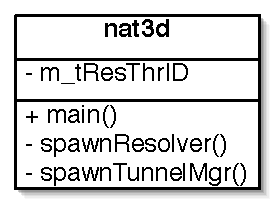
\includegraphics[width=0.4\textwidth]{figs/nat3d}
\end{center}
\caption{}
\label{fig:nat3d}
\end{figure}

This section describes the nat3d daemon component, which is described by Figure~\ref{fig:nat3d}.  This daemon is the actual NATTT
executable.  It runs 2 threads: one for the DNS resolver logic, and a second one that manages the IP tunnels.  This component is very
lightweight and is not responsible for much logic.


\subsection{Methods}

{\bf Public Methods}
\begin{itemize}
\item main(): This is the main method of the daemon.  It spawns a worker thread for the resolver and the directly calls the tunnel manager's
logic.
\item spawnResolver(): This method is uses as a callback to pthread\_create() and initializes and drives the DNS resolver logic.
\item spawnTunnelMgr(): This method initializes and drives the IP tunnel manager logic.
\end{itemize}

\subsection{Member Variables}
\begin{itemize}
\item m\_tResThrID: thread\_t This is the ID of the thread that runs the DNS logic.
\item m\_tTunThrID: thread\_t This type is reserved for the future and currently does not hold any information.
\end{itemize}
